\documentclass{report}

\input{~/latex/template/preamble.tex}
\input{~/latex/template/macros.tex}

\title{\Huge{Chapter 3 Notes}}
\author{\huge{Matt Warner}}
\date{\huge{}}
\pagestyle{fancy}
\fancyhf{}
\rhead{Math 211 - Calculus For Business \& Social Science}
\lhead{\leftmark}
\cfoot{\thepage}
% \usepackage[default]{sourcecodepro} \usepackage[T1]{fontenc}
\usepackage{pgfplots}
\pgfplotsset{compat=newest}
\pgfpagesdeclarelayout{boxed}
{
  \edef\pgfpageoptionborder{0pt}
}
{
  \pgfpagesphysicalpageoptions
  {%
    logical pages=1,%
  }
  \pgfpageslogicalpageoptions{1}
  {
    border code=\pgfsetlinewidth{1.5pt}\pgfstroke,%
    border shrink=\pgfpageoptionborder,%
    resized width=.95\pgfphysicalwidth,%
    resized height=.95\pgfphysicalheight,%
    center=\pgfpoint{.5\pgfphysicalwidth}{.5\pgfphysicalheight}%
  }%
}

\pgfpagesuselayout{boxed}

\begin{document}
  \maketitle
  \section*{3.1 - Using First Derivaties to Classify Maximum and Minimum Values}
  \bigbreak \noindent \bigbreak \noindent
  \hrule
  \bigbreak \noindent
  \vspace{-3mm}\subsection*{Increasing and Decreasing Functions}
  \bigbreak \noindent
  If the graph of a function rises from left to right over an interval $I$, the function is said to be increasing on, or over, $I$.
  \bigbreak \noindent
  If the graph drops from left to right, the function is said to be decreasing on, or over, $I$.
  \begin{figure}[ht]
  \centering
  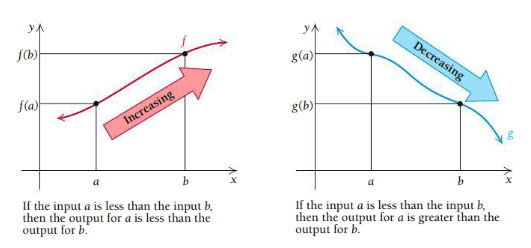
\includegraphics[width=0.65\textwidth]{  /home/mattw/niu/Math211/latexdocs/figures/paste.png}
  \end{figure}
\bigbreak \noindent
We can define these concepts as follows.
\begin{mdframed}
  \vspace{2mm}

  A function $f$ is \textbf{increasing} over $I$ if, for every $a$ and $b$ in $I$, 
  $$ \text{if } a < b, \ \ \ \text{then } f(a) < f(b)$$
  A function $f$ is \textbf{decreasing} over $I$ if, for every $a$ and $b$ in $I$,
  $$ \text{if } a < b, \ \ \ \text{then } f(a) > f(b)$$
\end{mdframed}
\bigbreak \noindent
The above definitions can be restated in terms of slopes of secant lines
\bigbreak \noindent
\hspace{35mm}Increasing: $\dfrac{f(b) - f(a)}{b - a} > 0$ \hspace{20mm} Decreasing: $\dfrac{f(b) -f(a)}{b - a} < 0$
\begin{figure}[ht]
\centering
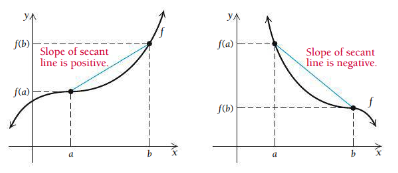
\includegraphics[width=0.65\textwidth]{ /home/mattw/niu/Math211/latexdocs/figures/second.png}
\end{figure}
\bigbreak \noindent
Since the derivative of a function tells us the slope of the tangent line to $f$ at any input x, we can also define an increasing or decreasing function using the derivative
\pagebreak
\thm{}{
  Let $f$ by differentiable over an open interval $I$
  \bigbreak \noindent
  If $f'(x) > 0$ for all x in $I$, then $f$ is increasing over $I$ 
  \vspace{2mm}

  If $f'(x) < 0$ for all $x$ in $I$, then $f$ is decreasing over $I$
}
\bigbreak \noindent
Theorem 0.1 is illustrated in the following graph of
$$ f(x) = \dfrac{1}{3}x^{3} - x + \dfrac{2}{3}$$
\begin{figure}[ht]
    \centering
    \incfig[1]{trialsiz}
    %\caption{trialsiz}
    %\label{fig:trialsiz}
\end{figure}
\bigbreak \noindent
Note in the graph above that x = -1 and x = 1 are not included in any interval over which the function is increasing or decreasing. These values are examples of \textit{critical values}
\bigbreak \noindent
\subsection*{Critical Values}
Consider the following graph
\begin{figure}[ht]
\centering
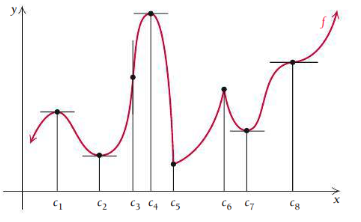
\includegraphics[width=0.5\textwidth]{ /home/mattw/niu/Math211/latexdocs/figures/critical.png }
\end{figure}
\bigbreak \noindent
Note the following
\begin{enumerate}
  \item $f'(x) = 0 \text{ for } x = c_1, c_2, c_4, c_7, \text{and }  c_8$. That is, the tangent line to the graph is horizontal at these values.
  \item $f'(x)$ does not exist for $ x = c_3, c_5$, and $C_6$. The tangent line is vertical at $c_3$, and there are corners at both $c_5$ and $c_6$.
\end{enumerate}
\pagebreak
\begin{mdframed}
  A \textbf{critical value}  of a function $f$ is any number $c$ in the domain of $f$ for which the tangent line at $(c,f(c))$ is \textbf{horizontal} or for which the derivative does not exist.
  \bigbreak \noindent
  That is, $c$ is a critical value if $f(c)$ exists and
  $$ f'(c) = 0 \ \ \ \text{or} \ \ \ f'(c) \text{ does not exist}$$
If $c$ is a critical value of a function $f$, then $(c,f(c))$ is a \textbf{critical point}
\end{mdframed}
Thus, in the graph of $f$ above:
\begin{itemize}
  \item $c_1, c_2,c_4,c_7,c_8$ are critical values because $f'(c) = 0$ for each value 
  \item $c_3,c_5,c_6$ are critical values because $f'(c)$ does not exist for each value
  \bigbreak \noindent
\end{itemize}
  \nt{
    A continuous function can change from increasing to decreasing or from decreasing to increasing \textbf{only} at a critical value.
  }
  \bigbreak \noindent
  \hrule
  \bigbreak
  \subsection*{Finding Relative Maximum and Minimum Values}
  Now consider a graph with ``peaks'' and ``valleys'' at $x = c_1, c_2, c_3, c_4$, and $c_5$
  \begin{figure}[ht]
  \centering
  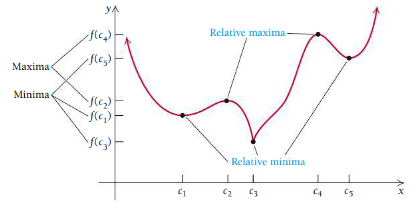
\includegraphics[width=0.5\textwidth]{ /home/mattw/niu/Math211/latexdocs/figures/peaks.png }
  \end{figure}
  \bigbreak \noindent
  Here, $f(c_2)$ and $f(c_4)$ are each an example of a \textbf{relative}, or \textbf{local, maximum}, and $f(c_1), f(c_3)$, and $f(c_5)$ are each an example of a \textbf{relative}, or \textbf{local minimum}.
  \bigbreak \noindent
  Collectively, maximum and minimum values are called \textbf{extrema}
  \nt{
  Note that it is possible for a relative minimum to be greater than a relative maximum.
  \bigbreak \noindent
  For example, $f(c_5) > f(c_2)$ in the graph in the next page.
  \bigbreak \noindent
  Also note that x-values at which a continuous function has relative extrema are those values for which the derivative is 0 or for which the derivative does not exist - the critical values
  }
  \pagebreak
  \thm{}{
    If a function $f$ has a relative extreme value $f(c)$ on an open interval, then $c$ is a critical value, and
    $$ f'(c) = 0 \ \ \ \text{or } \ \ f'(c) \text{ does not exist}$$
  }
\section*{Relative Extreme Points}

A relative extreme point, \( (c, f(c)) \), is higher or lower than all other points over an open interval containing \( c \).

\subsection*{Relative Minimum Point}

A relative minimum point, \( (c, f(c)) \), is lower than all other points over an open interval containing \( c \). Such a point has a \( y \)-value that is less than those of a neighborhood of points to the left and right of \( c \).

\subsection*{Relative Maximum Point}

Similarly, a relative maximum point, \( (c, f(c)) \), is higher than all other points over an open interval containing \( c \). This maximum point has a \( y \)-value that is greater than those of a neighborhood of points to the left and right of \( c \).

\textbf{Note:} In the preceding graph, \( (c_1, f(c_1)), (c_3, f(c_3)) \), and \( (c_5, f(c_5)) \) are all relative minimum points. Similarly, \( (c_2, f(c_2)) \) and \( (c_4, f(c_4)) \) are both relative maximum points.

\section*{Theorem 2}

\textit{Theorem 2 is useful and important to understand.} It states that to find relative extrema, we need only consider inputs for which the derivative is 0 or for which the derivative does not exist. Each critical value is a candidate for a value where a relative extremum might occur.

However, Theorem 2 does not guarantee that every critical value will yield a relative maximum or minimum. For instance, consider the graph of
\[
f(x) = (x-1)^3 + 2
\]
shown on the left. Note that:
\[
f'(x) = 3(x-1)^2 \quad \text{and} \quad f'(1) = 3(1-1)^2 = 0
\]
Thus, \( c = 1 \) is a critical value, but \( f \) has no relative maximum or minimum at that value. In fact, this function has no extrema anywhere.
\vspace{2mm}

\noindent Theorem 2 does guarantee that if a relative maximum or minimum occurs, then the first coordinate of that extremum is a critical value.
\bigbreak \noindent
The following graph leads us to a test.
\begin{figure}[ht]
\centering
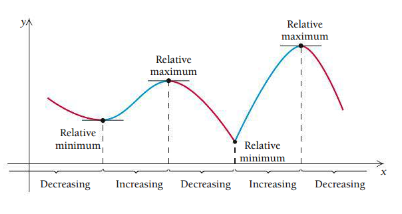
\includegraphics[width=0.58\textwidth]{ /home/mattw/niu/Math211/latexdocs/figures/test.png}
\end{figure}

\pagebreak
\begin{mdframed}
  \vspace{1.5mm}

Note that at a critical value where there is a relative minimum, the function $f$ is \textbf{decreasing} on the left of the critical value and \textbf{increasing} on the right.
\bigbreak \noindent
At a critical value where there is a relative maximum, the function $f$ is \textbf{increasing} on the left of the critical value and \textbf{decreasing} on the right. In both cases, the derivative changes signs on either side of the critical value.
\vspace{1.5mm}
\end{mdframed}
\bigbreak \noindent \bigbreak \noindent \bigbreak \noindent \bigbreak \noindent 
\begin{figure}[ht]
\centering
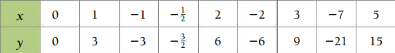
\includegraphics[width=0.9\textwidth]{ /home/mattw/niu/Math211/latexdocs/figures/table.png }
\end{figure}

\pagebreak
\noindent
Derivatives can tell us when a function is increasing or decreasing. This leads us to the First-Derivative Test.
\thm{}{
  For any continuous function $f$ that has exactly one critical value $c$ in an open interval $(a,b)$
  \bigbreak \noindent
  \textit{\textbf{F1.}} $f$ has a relative minimum at $c$ if $f'(x) < 0$ on $(a,c)$ and $f'(x) > 0$ on $(c,b)$. That is, $f$ is decreasing to the left of $c$ and increasing to the right of $c$
  \bigbreak \noindent
  \textit{\textbf{F2}} $f$ has a relative maximum at $c$ if $f'(x) > 0$ on ($a,c$) and $f'(x) < 0$ on ($c,b$). That is, $f$ is increasing to the left of $c$ and decreasing to the right of $c$
  \bigbreak \noindent
  \textit{\textbf{F3}} $f$ has neither a relative maximum nor a relative minimum at $c$ if $f'(x)$ has the same sign on $(a,c)$ as on $(c,b)$
  \bigbreak \noindent
  We can use the First-Derivative Test to find relative extrema.
}
\q
Consider the function $f$ given by
$$ f(x) = 4x^3 - 9x^2 - 30x + 25$$
\bigbreak \noindent
\textbf{Find any relative exterma}
\bigbreak \noindent
\textit{\textbf{Find the derivative}}

$$ \frac{d}{dx}[4x^3] - \frac{d}{dx}[9x^2] - \frac{d}{dx}[30] + \frac{d}{dx}[25]$$

$$ f'(x) = 12x^2 - 18x -30$$
\textit{\textbf{set f'(x) = 0}}

$$ 12x^2 -18x - 30 = 0$$
\textit{\textbf{divide both sides by 6}}
$$ 2x^2 - 3x -5 = 0$$
$$ (x+1)(2x-5) = 0$$
$$ x = -1 \ \ \ \ or \ \ \ \ x = \dfrac{5}{2}$$
The critical values are -1 and $\dfrac{5}{2}$. Since it is at these values that a relative maximum or minimum might exist, we examine the sign of the derivative on the intervals
$$ (-\infty, -1), (-1,\dfrac{5}{2}), (\dfrac{5}{2}, \infty)$$
To do so, we select a convenient test value in each interval and evalulate f'(x). 
\bigbreak \noindent
\textit{\textbf{Let's use the values: -2, 0, 4}}
$$ f'(-2) = 54$$
$$f(0) = -30$$
$$ f(4) = 90$$
\textit{\textbf{Result:}} \\

\noindent $f$ is increasing on $(-\infty, -1)$ \\
$f$ is decreasing on $(-1, \dfrac{5}{2})$ \\
$f$ is increasing on $(\dfrac{5}{2}, \infty)$ 
\bigbreak \noindent
By the First-Derivative Test, $f$ has a relative maximum at $x = -1$ and a relative minimum at $ x=\dfrac{5}{2}$
\bigbreak \noindent
The value of the relative maximum is given by
$$ f(-1) = 4(-1)^3 - 9(-1)^2 - 30(-1) + 25$$
$$ f(-1) = 42 $$
The value of the relative minimum is given by
$$ f(\frac{5}{2}) = 4(\frac{5}{2})^3 - 9(\frac{5}{2})^2 - 30(\frac{5}{2}) + 25$$
$$ f(\frac{5}{2}) = -\dfrac{175}{4} $$
\bigbreak \noindent
Thus, there is a relative maximum point at $(-1,42)$ and a relative minimum point at $(\frac{5}{2}, -\frac{175}{4})$
\bigbreak \noindent
\begin{center}
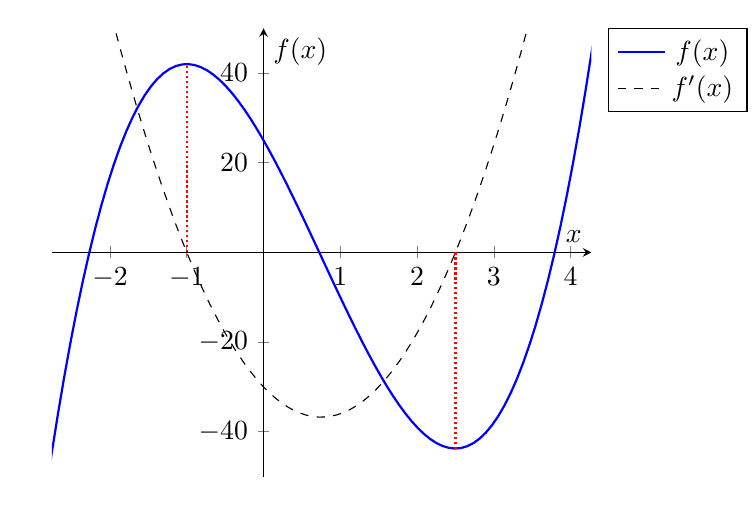
\begin{tikzpicture}
    \begin{axis}[
        axis lines = middle,
        xlabel = \(x\),
        ylabel = \(f(x)\),
        domain=-3:5,
        samples=100,
        ymin=-50,
        ymax=50,
        legend pos=outer north east,
    ]
    
    % Plotting f(x)
    \addplot[color=blue, thick]{4*x^3 - 9*x^2 - 30*x + 25};
    \hspace{3mm}\addlegendentry{\(f(x)\)}
    % Plotting f'(x)
    \addplot[color=black, dashed]{12*x^2 - 18*x - 30};
    \addlegendentry{\(f'(x)\)}
    % Marking and drawing vertical dashed lines for the critical points
    \draw [densely dotted, red, thick] (axis cs: -1,0) -- (axis cs: -1,{4*(-1)^3 - 9*(-1)^2 - 30*(-1) + 25});
    \draw [densely dotted, red, thick] (axis cs: 5/2,0) -- (axis cs: 5/2,{4*(5/2)^3 - 9*(5/2)^2 - 30*(5/2) + 25});
    \end{axis}
\end{tikzpicture}
\end{center}
\bigbreak \noindent
\nt{
  Note that $f'(x) = 0$ where $ f(x)$ has relative extrema. We summarize the behavior of this function by noting where it is increasing or decreasing and by characterizing its critical points
  \bigbreak \noindent
  \begin{itemize}
    \item $f$ is increasing over the interval $(-\infty, -1$) 
    \item $f$ has a relative maximum point at $(-1,42)$
    \item $f$ is decreasing over the interval $(-1,\dfrac{5}{2})$
    \item $f$ has a relative minimum point at $(\dfrac{5}{2}, -\dfrac{175}{4})$
    \item $f$ is increasing over the interval $(\dfrac{5}{2}, \infty)$
  \end{itemize}
}
\bigbreak \noindent
To use the first derivative for graphing a function $f$
\begin{enumerate}
  \item Find all critical values by determining where $f'(x)$ is 0 and where $f'(x)$ is undefined (but $f(x)$ is defined). Find $f(x)$ for each critical value
  \item Use the critical values to divide the x-axis into intervals and choose a test value in each interval
  \item Find the sign of $f'(x)$ for each test value chosen in step 2, and use this information to determine where $f$ is increasing or decreasing and to classify any extrema as relative maxima or minima
  \item Plot some additional points and sketch the graph
\end{enumerate}

\pagebreak
\q
Find the relative extrema and sketch the graph of the function $f$ given by
$$ f(x) = 2x^3  - x^4$$
\textit{\textbf{We first need to take the derivative}}
$$ f'(x) = \frac{d}{dx}2x^3 - \frac{d}{dx}x^4$$
$$ f'(x) = 6x^2 - 4x^3$$
\textit{\textbf{Find the critical values}}

$$ 6x^2 - 4x^3$$
$$ = 2x(3-2x)$$
$$ 2x^2 = 0 \ \ \ \ 3 - 2x = 0$$
$$ x = 0 \ \ \ \ x = \dfrac{3}{2}$$
\textit{\textbf{So, the intervals are}}

$$ (-\infty,0), \ \ \ (0,\dfrac{3}{2}), \ \ \ (\dfrac{3}{2}, \infty)$$
\bigbreak \noindent
\textit{\textbf{Choose test values within the intervals to see where its increasing / decreasing}}
$$(-\infty, 0): \text{ Test } -1, \ \ \ f'(-1) = 6(-1)^2 - 4(-1)^3 = 6 + 4 = 10 > 0$$
$$ (0,\dfrac{3}{2}): \text{ Test } 1 \ \ \ f'(1) = 6(1)^2-4(1)^3 = 6 -4 = 2 > 0$$
$$ (\dfrac{3}{2}): \text{ Test } 2 \ \ \ f'(2) = 6(2)^2 -4(2)^3 = 24 -32 = -8 < 0$$
\bigbreak \noindent
The relative maxima / minima would be at the critical values: 0, $\dfrac{3}{2}$
\bigbreak \noindent
Since $f$ in increasing on both sides of 0, there is no extremum there.
There is however, a maximum at $ x = \dfrac{3}{2}$ Thus, 
$$ f\left(\dfrac{3}{2}\right) = 2\left(\dfrac{3}{2}\right)^3 - \left(\dfrac{3}{2}\right)^4$$
$$ = 2 \cdot \dfrac{27}{8} - \dfrac{81}{16}$$
$$ \dfrac{108}{16} - \dfrac{81}{16} = \dfrac{27}{16}$$
\bigbreak \noindent
So, there is a Relative maximum at
$$ \left(\dfrac{3}{2}, \dfrac{27}{16}\right)$$
\bigbreak \noindent
So,
\begin{itemize}
  \item $f$ is increasing over the interval $(-\infty, 0)$
  \item $f$ has a critical value at x = 0, but the critical point (0,0) is neither a minimum nor a maximum
  \item $f$ is increasing over the interval $(0,\dfrac{3}{2})$
  \item $f$ has a relative maximum at the point $ \left(\dfrac{3}{2}, \dfrac{27}{16}\right)$
  \item $f$ is decreasing over the interval $(\dfrac{3}{2},\infty)$
\end{itemize}

\pagebreak
\section*{3.2 - Using Second Derivatives to Classify Maximum and Minimum Values and Sketch Graphs}
\bigbreak \noindent
The graphs of two continous functions are shown Below. The graph of $f$ bends upwards and the graph of $g$ bends downwards. Let's relate these observations to each function's derivative.
\bigbreak \noindent
We draw tangent lines moving along the graph of $f$ from left to right. What happens to the slopes of the tangent lines? We do the same for the graph of $g$. Is there a relationship between the changing slopes and the way the graph bends?
\bigreak \noindent

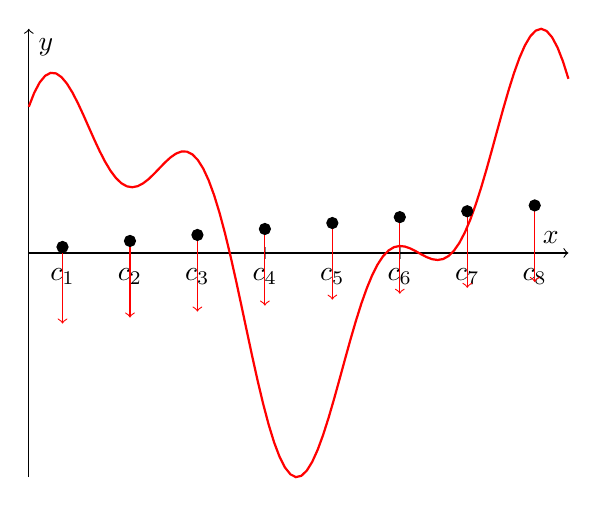
\begin{tikzpicture}
\begin{axis}[
    axis lines=middle,
    axis line style={->},
    xlabel={$x$},
    ylabel={$y$},
    xtick={1,2,3,4,5,6,7,8},
    xticklabels={$c_1$,$c_2$,$c_3$,$c_4$,$c_5$,$c_6$,$c_7$,$c_8$},
    ytick=\empty,
    domain=0.5:8.5,
    samples=100,
    clip=false,
]

% Define the function f(x)
\addplot[red, thick] {sin(deg(x)) + 0.5*sin(deg(2.5*x))};
\addplot[only marks, mark=*, mark options={fill=black}] coordinates {(1,{sin(1)+0.5*sin(2.5*1)}) (2,{sin(2)+0.5*sin(2.5*2)}) (3,{sin(3)+0.5*sin(2.5*3)}) (4,{sin(4)+0.5*sin(2.5*4)}) (5,{sin(5)+0.5*sin(2.5*5)}) (6,{sin(6)+0.5*sin(2.5*6)}) (7,{sin(7)+0.5*sin(2.5*7)}) (8,{sin(8)+0.5*sin(2.5*8)})};

% Add arrows at critical points
\foreach \x in {1,2,...,8}{
    \edef\temp{\noexpand\draw[->, red] (axis cs:\x,{sin(\x)+0.5*sin(2.5*\x)}) -- (axis cs:\x,{sin(\x)+0.5*sin(2.5*\x)-0.5});}
    \temp
}

\end{axis}
\end{tikzpicture}
\end{document}
